\setlength{\footskip}{8mm}

\chapter{Analytics in financial institutions}

\section{Why?}
According to a joint research study, by Boston Consulting Group and Morgan Stanley with analytics professionals, it was reveled that the financial institutions lagged behind other verticals in the use of data analytics~\shortcite{BCGanalytics2017} and it is shown in figure~\ref{fig:da_digitization}. One of the findings of the research was that FI's are investing a lot of capital, an estimated total of about \textdollar1bn. In addition it was found that for near term value creation the FI's expected data analytics to optimize customer acquisition, customer retention, operational efficiency, and risk mitigation.
\newline
\newline
\begin{figure}[H]
	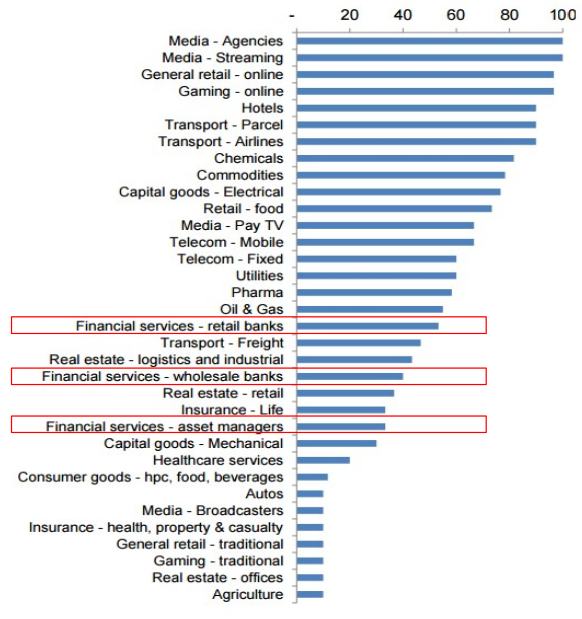
\includegraphics[scale = 0.7]{figures/DA_used_verticals.png}
	\caption{Reprinted from the Morgan Stanley Digitization Index ranks }
	\label{fig:da_digitization}
\end{figure}
\FloatBarrier

\newpage
\section{State of analytics in financial companies}
From the survey of FI's, a mix of interviewees representing payment companies, service providers, insurance, commercial banks, BCG made some interesting discoveries. It was found that most organizations have invested in analytics techniques to generate market perceptions. Some of the most used were those of social media, log, text and location analytics as shown in figure~\ref{fig:da_capabilities}.

\begin{figure}[H]
	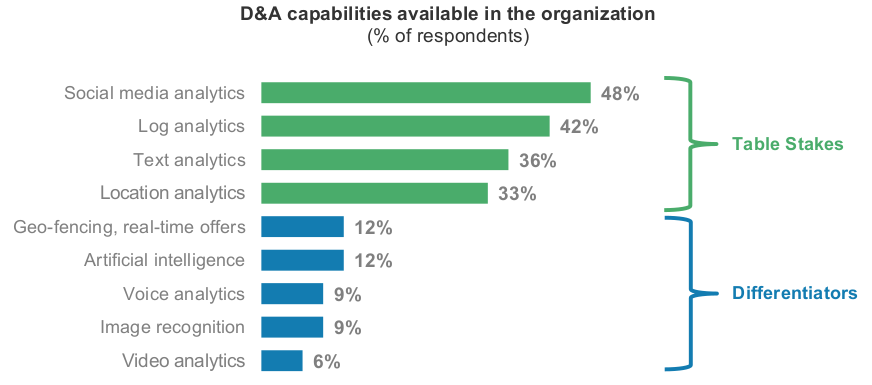
\includegraphics[scale = 0.5]{figures/DA_capabilities.png}
	\caption[Da capablities]{Reprinted from the work of Boston consulting group  }
	\label{fig:da_capabilities}
\end{figure}
\FloatBarrier

Researchers have highlighted that most of the interviewees claimed that institutions are yet to make substantial gain from investments in analytics. They identified that companies can make gains from automation and digitization of manual processes. Additionally, it was noted that financial institutions are adopting digital processes to automate data collection for KYC (Know Your Customer) service and Anti-money laundering 
%\newline
%\newline
Customers are loyal consumers of products, which give value for their monetary investments. Big institutions tend to over look the need for value creation and focus their analytics and metrics to improve profit \shortcite{Reichheld1996}. In the HBR report Reichheld makes certain  observations that customers of large companies witness degrading value standards and secondly increasing rate of customer churn is a good variable to predict cash flow from consumer to company. He also noted that companies can replace old customer with new ones but the profits are lower as cost of induction is high.

\newpage
\section{Challenges faced by analytics}
For every new technology there are certain common challenges, such as those of acceptability and usability. Finding out the actual benefit or Return on investment for newer technologies and solutions such as those of digital assistants remains a mystery. There is no quantifiable or tangible benefit, but only a perception that it could revolutionize the method of banking and investing.
Some hurdles, such as of vision, budget, and getting all members on board, are faced early in the life-cycle of adopting such bold complex projects. Institution leadership faces the tough task of decision making and if rests on them to perceive value at the end of project.
Even after adopting analytics and tools, management faces challenges of educating shareholders, staff and customers to be literate enough to invest and interact with solutions for effective usage.




\chapter{Descriptive Techniques} 
\label{ch:literature-review}

The sole purpose of using the methods in this category would be to describe the Hypothesis. Descriptive analytics or data mining are at the bottom of the big data value chain, but they can be valuable for uncovering patterns that offer insight. A simple example of descriptive analytics would be assessing credit risk; using past financial performance to predict a customer’s likely financial performance. Descriptive analytics can be useful in the sales cycle, for example, to categorize customers by their likely product preferences and sales cycle.

To summarize data into meaningful charts and reports, for example, about budgets, sales, revenues, or cost. They allow managers to obtain standard and customized reports, and drill down into the data and to make queries to understand the impact of an advertising campaign, for example, review business performance to find problems or areas of opportunity, and identify patterns and trends in data. Typical questions that descriptive analytics help answer are: How much did we sell in each region? What was our revenue and profit last quarter? How many and what types of complaints did we resolve? Which factory has the lowest productivity? Descriptive analytics also help companies to classify customers into different segments, which enable them to develop specific marketing campaigns and advertising strategies. [1]

There are two main approaches to apply in this topic Data warehousing and Visual analytics with reporting.

Descriptive analytics is very common and basic form of data mining technique to derive meaning and trend from data. Almost all of the companies in financial sector utilize the tools based on these techniques. The techniques in this are relatively basic compared with those of predictive models and prescriptive models. Institutions generally use tools which can generate reports regularly, some are printed monthly while some others are generated  as a yearly routine. Such demands for reports describe the status quo of the balance sheets, organizational debts and cash flows. Daly transactions and updates of balances are maintained in the books or accounts and reports are generated daily for accountants and auditors. Thus it is imperative that vital functions of reporting, updating and auditing are functionalities of some business analytics.

There are several techniques employed by businesses to analyze and display data. They are as follows:
\begin{enumerate}
	\item OLAP
	\item Datawarehouse
	\item Graphical views
	\item Performance dashboard and KPI's
\end{enumerate}

\section{Social media analytics}

\section{Log analytics}


\section{Text analytics}
In a paper titled ``When machines read the news``~\shortcite{gross2011machines}, the authors have used text mining to derive the relation between scrip news and intra-day stock trading. They try to relate the stock price fluctuations and liquidity, to the unscheduled news flash. The researchers used Reuter`s NewScope is an news engine which classifies stock/company related news into positive, negative and neutral segments. The techniques used was VAR model known as vector autoregressive model. This model is used for multivariate time series. 
The data was sourced from Reuter`s NewsScope sentiment engine. It contains around 29,500 records of news headlines in the period of 1 year from the month of July 2007 to June 2008. Each news item has 3 attributes of sentiment, relevance and novelty. 40 stocks listed on the London stock exchange were selected for analysis. These are actively traded on the exchange and thus a dynamic market sentiment and frequent news coverage. These stocks cover about 70\% of the FTSE100 market capitalization. 


\section{Location analytics}



%
%
%
%

\setlength{\footskip}{8mm}

\chapter{Predictive Techniques} 
\label{predictive-techniques}

Predictive analytics use big data to identify past patterns to predict the future. For example, some companies are using predictive analytics for sales lead scoring. Some companies have gone one step further use predictive analytics for the entire sales process, analyzing lead source, number of communications, types of communications, social media, documents, CRM data, etc. Properly tuned predictive analytics can be used to support sales, marketing, or for other types of complex forecasts.


The basis of Predictive modeling is the use of data mining techniques to forecast future results. Data mining is the process of sorting data to find patterns or infer relationships.
Thus a formulation of a statistical model with relevant variables is essential for prediction. 
ref from site (http://searchdatamanagement.techtarget.com/definition/predictive-modeling) and (http://searchsqlserver.techtarget.com/definition/data-mining)

Data mining techniques are used in credit card systems to detect fraud, in loan approval systems, identifying customer types and targeting specific promotional schemes. It is used to model customer behavior and detect churning to certain financial products. Insurance schemes and bank deposits are volatile instruments due to the uncertainty of the free economy. site (https://hbr.org/1996/03/learning-from-customer-defections).


There are many techniques to modeling predictive analytics 


\begin{enumerate}
	\item Clustering methods
	\item Regession methods
	\item Classification methods
	\item Association rules
\end{enumerate}e)

%
%
%
%
\section{Geo fencing}
Geo-fencing (or also known as Location Analytics) is the term for creating a location based analytics algorithm which can track customers in a certain area and deliver valuable marketing or services. The technology works based on geographic location services and tracks any potential clients with their mobile gps. 
Geo fencing tools are software applications which reside on the 

Use-cases for geofencing :
\begin{itemize}
	\item Manage a group of cargo vehicles
	\item Detect and optimize harbor docking for port management of ships
	\item Density flow of vehicles and management on roads or air space near airports.
	\item Exhibition centers can manage the flow of attendees to optimally view all exhibits, ensuring all items on display can be viewed.
	\item Shopping malls and shops can monitor the passage of people and optimize the display of commercials or products.
\end{itemize}

Geo fences are designed into the application which generally store the latitude and longitudes of the location to be monitored. When the user uses the app, it reads data from the gps module and keeps checking if the client has crossed any geo fence en-route. Now-a-days geo fencing.

Google maps geo fencing is available via API's 

\newpage
\section{Artificial intelligence}
AI was developed a long time ago, but it has for recent years gained much traction and entered our lives. AI was present from the 1950's, but it has only gained popularity.
According to an article by PwC~\shortcite{PwcAI2017}, some companies have invested in AI, Machine and Cognitive learning tools and have implemented solutions for Chatbots, Personal assistants etc. Big data coupled with faster computing and ubiquitous implementation with cloud computing has certainly boosted research and development.
As per a Forbes research projection, in the next 10 years, implementations of AI will increase economic growth by 100\% in about 20 countries. Also there could be an increase in productivity of around 40\% of banks financial labor~\shortcite{Forbes2017}.

AI is used as a technique to automate various categories of tasks such as following~\shortcite{rich1991artificial} :
\begin{itemize}
	\item Mundane tasks
		\begin{itemize}
			\item Perception via Vision and Speech
			\item Natural language processing 
			\item Robot control and common sense
		\end{itemize}
	\item Formal tasks
	\begin{itemize}
		\item Playing games such as chess, go, checkers etc
		\item Solving mathematical problems of geometry, logic, calculus
	\end{itemize}
	\item Expert tasks
	\begin{itemize}
		\item Engineering design, fault finding, Manufacturing planning
		\item Scientific analysis
		\item Medical diagnosis
		\item Financial analysis
	\end{itemize}
\end{itemize}

Some techniques which fall in the space of AI are Support vector machines, Heuristics, Neural networks, Markhov decision process, and NLP natural language processing.

In an example case presented by a researcher from Romania~\shortcite{Costea2014}, the techniques of artificial intelligence combined with fuzzy logic for classification.
The case is applied to a scenario where the National Bank of Romania classifies NFI`s into ``good`` or ``poor`` depending on the periodic financial reporting. The Non - Banking financial institutions of Romania are regulated by governmental policy to send their financial reports to the NBR for scrutiny. NBR appoints their staff to manually screen the reports and classify for goodness or badness and then need to proceed for on site inspection.
The artificial neural network is built with genetic algorithm and trained to perform classification. The process involved introducing mutations to chromosomes of both the parents and offspring.

The dataset is made of 990 records having 11 attributes grouped into 3 dimensions viz., Capital adequacy, assets` quality and profitability. The data ranged between 2007 to 2012. There were 68 non banking financial institutions. 4 clusters were chosen using the Fuzzy C Means algorithm. The ANN structure contained 8 neurons on the first hidden layer and 5 on the next. The accuracy rate achieved was around 92.32\% and validation accuracy around 91\% and testing accuracy about 89\%. Thus in this study the researcher was able to get high accuracy artificial neural network classification to classify the financial statements of non- banking institutions in Romania.


\section{Deep learning}
In the paper ref~\shortcite{heaton2016deep} the authors have presented a list of techniques which are being used to classify and predict financial domain problems ranging from :
\begin{itemize}
	\item securities pricing
	\item portfolio design and entity selection
	\item risk management
\end{itemize}.

Deep learning models are being used in financial product design by working with big data. These models produce better results than the traditional techniques of economics. 

\section{Voice analytics}



\section{Image recognition}



\section{Video analytics}



\setlength{\footskip}{8mm}


\newpage
\section{Combating financial fraud}
In a research~\shortcite{Chen2015} , the Alibaba company developed an analytics solution to tackle fraud in the company. Big data from the company was leveraged to study patterns of financial transactions, user behavior and network analysis to predict in real time with machine learning algorithm, predicting bad user`s and transactions. AntBuckler is a predictive analytics solution developed in-house to detect and prevent fraudulent transactions. Big data center of Alibaba use many fraud risk models to deal with activities. They apply the fraud and risk models on all processes related to account opening, identity verification, order placement. AntBuckler generates RAIN score - risk score for merchants and shared with banks, merchants for their judgment on risk levels.
\newline
Shown below is the framework Alibaba uses in Alipay~\ref{fig:alipay}.

\begin{figure}[H]
	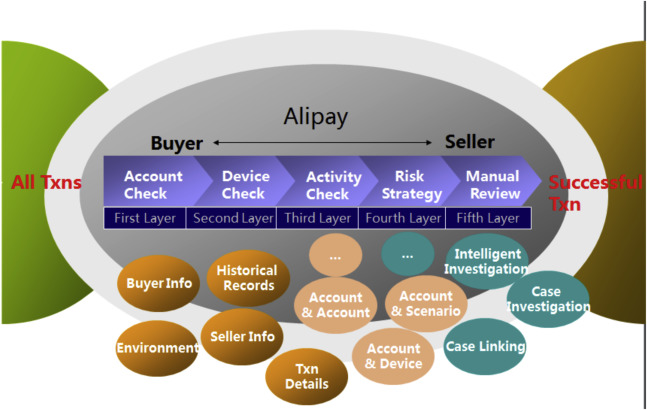
\includegraphics[scale = 0.8]{figures/alipay.jpg}
	\centering
	\caption{Fraud analytics in Alipay}
	\label{fig:alipay}
\end{figure}

Stages of fraud restrictions :
\begin{itemize}
	\item Account check
	\item Device check
	\item Activity check
	\item Risk strategy 
	\item Manual review
\end{itemize}

RAIN - model used by Alibaba stands for Risk of activity, identity and network~\ref{fig:rain_dimension}. It identifies the risk of any object interacting with the Alibaba system such as a human, credit card or account. 3 dimension are defined in the system viz., activity, identity and network; and all variables are classified into them, values of variables are computed for all the objects. Depending upon the scenario particular variables are chosen and RAIN score is computed. Such as in the case of credit card fraud, identity variables are adjusted with higher weights; in the case of credit scoring network group of variables are weighted more. Logistic regression part of a Machine learning is used to determine the weights for a given scenario.

\begin{figure}[H]
	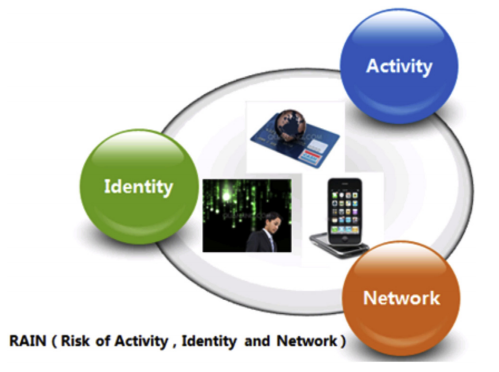
\includegraphics[scale = 0.8]{figures/RAIN_dimension.png}
	\centering
	\caption{Dimensions of RAIN score}
	\label{fig:rain_dimension}
\end{figure}

Network based graph representation is also used to link accounts and ip addresses to visually represent the links between name, address, phone, credit card, etc.

\chapter{Prescriptive Techniques}
\label{prescriptive-techniques}

Prescriptive analytics is really valuable, but largely not used. According to Gartner, 13 percent of organizations are using predictive but only 3 percent are using prescriptive analytics. Where big data analytics in general sheds light on a subject, prescriptive analytics gives you a laser-like focus to answer specific questions. For example, in the health-care industry, you can better manage the patient population by using prescriptive analytics to measure the number of patients who are clinically obese, then add filters for factors like diabetes and LDL cholesterol levels to determine where to focus treatment. The same prescriptive model can be applied to almost any industry target group or problem.




%
%
%
%

\setlength{\footskip}{8mm}

\chapter{Optimization Techniques} 
\label{optimization-techniques}





%
%
%
%

\setlength{\footskip}{8mm}

\chapter{Visualization Techniques} 
\label{visualization-techniques}





%
%
%
%

\setlength{\footskip}{8mm}

